\documentclass[a4paper,12pt]{article}
\usepackage{amsmath, amsthm}
\usepackage{datetime}
\usepackage{framed}
\usepackage{enumitem}
\usepackage{fancyref}
\usepackage{wrapfig}
\usepackage{pifont}

\usepackage{tikz}
\usetikzlibrary{fit,arrows,calc}

\usepackage{csquotes}
\renewcommand{\mkbegdispquote}[2]{\itshape}

\newdateformat{nianyueri}{ \THEYEAR 年 \THEMONTH 月 \THEDAY 日 }

\usepackage{xstring}
\usepackage{catchfile}
\CatchFileDef{\HEAD}{../.git/refs/heads/master}{}
\newcommand{\gitrevision}{%
  \StrLeft{\HEAD}{7}%
}

\usepackage{data/circledsteps}
\usepackage[top=1in,bottom=1in,left=1in,right=1in]{geometry} % 用于设置页面布局
\usepackage{xeCJK} % 用于使用本地字体
\usepackage[super, square, sort&compress]{natbib} % 处理参考文献
\usepackage{titlesec, titletoc} % 设置章节标题及页眉页脚
%\usepackage{xCJKnumb} % 中英文数字转换
\usepackage{amssymb}
\usepackage{amsmath} % 在公式中用\text{文本}输入中文
\usepackage{diagbox}
\usepackage{multirow} % 表格中使用多行
\usepackage{booktabs} % 表格中使用\toprule等命令
\usepackage{rotating} % 使用sidewaystable环境旋转表格
\usepackage{tabularx}
\usepackage{graphicx} % 处理图片
\usepackage{footnote} % 增强的脚注功能,可添加表格脚注
\usepackage{threeparttable} % 添加真正的表格脚注,示例见README
\usepackage{hyperref} % 添加pdf书签

\usepackage{tikz}
\usetikzlibrary{shapes,arrows,shadows}

% 字体设置
\setmainfont{Times New Roman}
\setsansfont[Scale=MatchLowercase,Mapping=tex-text]{PT Sans}
\setmonofont[Scale=MatchLowercase]{PT Mono}
\setCJKmainfont[ItalicFont={Kaiti SC}, BoldFont={Heiti SC}]{Songti SC}
\setCJKsansfont{Heiti SC}
\setCJKmonofont{Songti SC}
% \setCJKmainfont[BoldFont={FZXiaoBiaoSong-B05S}]{Songti SC}
% \setCJKfamilyfont{kai}[BoldFont=Heiti SC]{Kaiti SC}
% \setCJKfamilyfont{song}[BoldFont=Heiti SC]{Songti SC}
% \setCJKfamilyfont{hei}[BoldFont=Heiti SC]{Heiti SC}
% \setCJKfamilyfont{fsong}[BoldFont=Heiti SC]{Songti SC}
% \newcommand{\kai}[1]{{\CJKfamily{kai}#1}}
% \newcommand{\hei}[1]{{\CJKfamily{hei}#1}}
% \setromanfont[Mapping=tex-text]{TeXGyrePagella}
% \setsansfont[Scale=MatchLowercase,Mapping=tex-text]{TeXGyrePagella}
% \setmonofont[Scale=MatchLowercase]{Courier New}
%%设置常用中文字号,方便调用
\newcommand{\erhao}{\fontsize{22pt}{\baselineskip}\selectfont}
\newcommand{\xiaoerhao}{\fontsize{18pt}{\baselineskip}\selectfont}
\newcommand{\sanhao}{\fontsize{16pt}{\baselineskip}\selectfont}
\newcommand{\xiaosanhao}{\fontsize{15pt}{\baselineskip}\selectfont}
\newcommand{\sihao}{\fontsize{14pt}{\baselineskip}\selectfont}
\newcommand{\xiaosihao}{\fontsize{12pt}{\baselineskip}\selectfont}
\newcommand{\wuhao}{\fontsize{10.5pt}{\baselineskip}\selectfont}
\newcommand{\xiaowuhao}{\fontsize{9pt}{\baselineskip}\selectfont}
\newcommand{\liuhao}{\fontsize{7.5pt}{\baselineskip}\selectfont}

% 章节标题显示方式及页眉页脚设置
% \item xCJKnumb是自己额外安装的包
% \item titleformat命令定义标题的形式
% \item titlespacing定义标题距左、上、下的距离
\titleformat{\section}{\raggedright\large\bfseries}{\thesection}{1em}{}
\titleformat{\subsection}{\raggedright\normalsize\bfseries}{\thesubsection}{1em}{}
\titlespacing{\section}{0pt}{*0}{*2}
\titlespacing{\subsection}{0pt}{*0}{*1}
% 由于默认的2em缩进不够,所以我手动调整了,但是在windows下似乎2.2就差不多了,或者是article中没有这个问题
\setlength{\parindent}{2.2em}

% 设置表格标题前后间距
\setlength{\abovecaptionskip}{0pt}
\setlength{\belowcaptionskip}{0pt}


\renewcommand{\refname}{\bfseries{参~考~文~献}} %将Reference改为参考文献(用于 article)
% \renewcommand{\bibname}{参~考~文~献} %将bibiography改为参考文献(用于 book)
\renewcommand{\baselinestretch}{1.38} %设置行间距
\renewcommand{\figurename}{\small\ttfamily 图}
\renewcommand{\tablename}{\small\ttfamily 表}


\usepackage{stmaryrd}
\usepackage{mathtools}

\xeCJKsetwidth{‘’“”}{1em}

\usepackage[acronym,xindy]{glossaries}
\renewcommand*{\glossaryname}{术~语~列~表}
\makeglossaries

\usepackage[xindy]{imakeidx}
\makeindex

\loadglsentries[main]{glossary}

\title{有效过程与自然法则}
\date{1985 年 9 月 9 日}
\author{罗伯特·罗森}

\begin{document}
\maketitle{}
\centerline{\rule{13cm}{0.4pt}}

\centerline{ 苑明理(翻译) }
\centerline{ 杨文波(校读) }
\centerline{ 第 \space\gitrevision\space 版}
\centerline{ \nianyueri\today }

\centerline{\rule{13cm}{0.4pt}}
\renewcommand{\contentsname}{\hfill\bfseries 目录\hfill}
\setcounter{tocdepth}{2}
\tableofcontents
\centerline{\rule{13cm}{0.4pt}}
\newpage

\section{引言}

现代科学史上最引人注目的思想交汇之一,发生在 1931 年哥德尔关于形式不可判定性原始论文发表\footnote[1]{译注:即\cite{GodelK1931}}
与 1943 年麦卡洛克和皮茨关于神经网络著作\footnote[2]{译注:McCulloch, W. and W. Pitts. “A logical calculus of the ideas immanent in nervous activity.” Bulletin of Mathematical Biology 52 (1943): 99-115.}发表之间的短短几年间。
在这十二年中,逻辑学、数学、大脑理论和数字计算的可能性之间建立了基本的相互关系,现在想起来所有这些仍然让人叹为观止。
人们当时认为,半个世纪之后的今天依然认为,这些思想预示着一场革命,恰如三个世纪前牛顿所取得的进展一样根本性的革命。

\begin{figure}[ht]
\centering
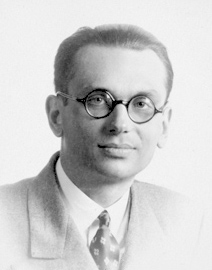
\includegraphics[height=1.5in]{images/kurt_godel.jpg}
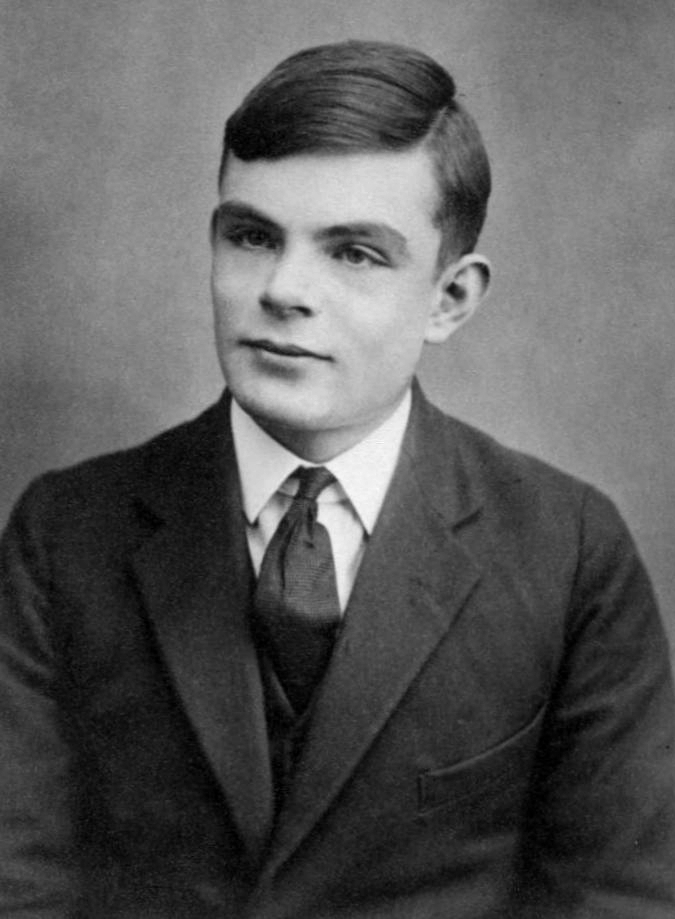
\includegraphics[height=1.5in]{images/alan_turing.jpg}
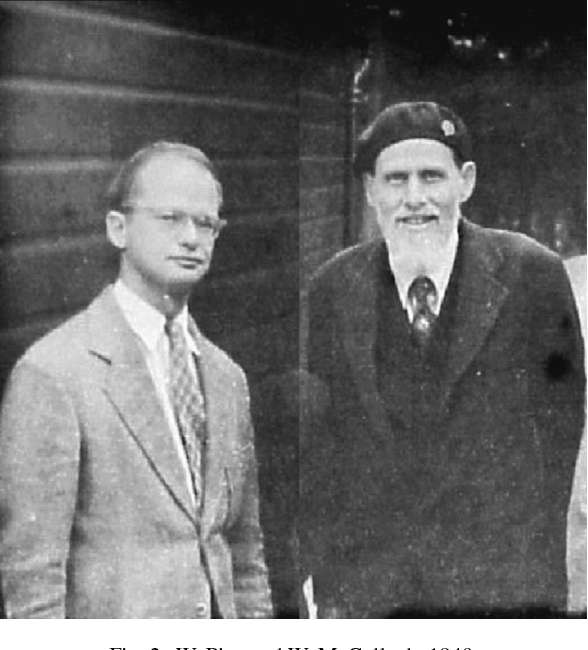
\includegraphics[height=1.5in]{images/pitts_mcculloch_1949.png}
\caption{青年哥德尔;青年图灵;皮茨和麦卡洛克的合照}
\end{figure}

阿兰·图灵的名字在这些惊人发展的历史上是非凡的。正因为图灵,在他 1936 年发表的开创性论文\footnote[3]{译注:即\cite{TuringA1937}}中,通过构建以他的名字命名的“机器”类,他首次把这些相关的思想真正并列在一起。
首先,\emph{\gls{图灵机}}是从人类进行数学计算的心理过程中明确推演出来的;其次,它们代表了逻辑或算法过程的形式化体现,如同在数学中的表现;
再则,通过使用“机”这个术语,它们又代表了,利用物质过程来扩展我们自己的数学能力(很快会通过数字计算机的发明来实现),并且在更深的层次上,为探索生命本身建立一个新的、强大的隐喻。

\begin{figure}[ht]
\centering
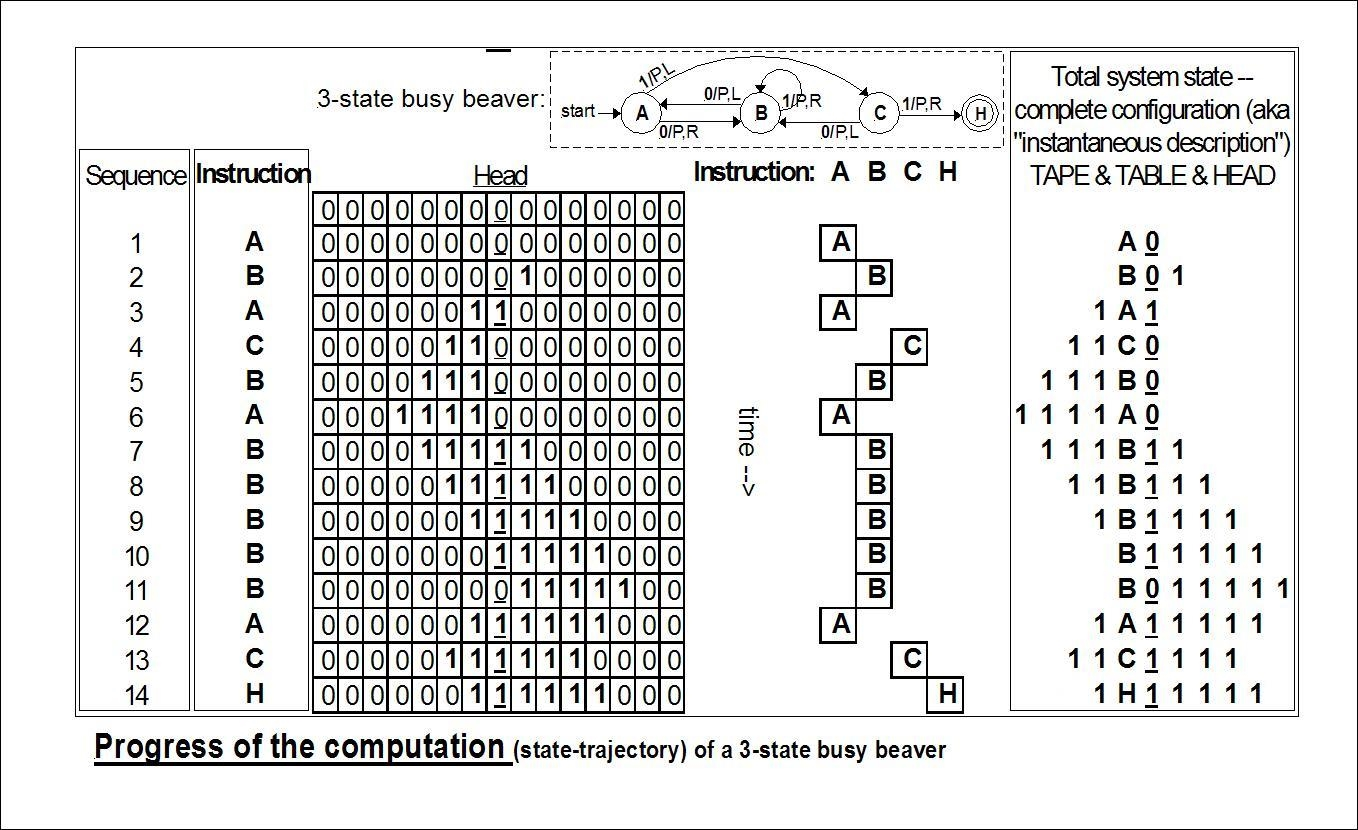
\includegraphics[height=2.0in]{images/turing_machine.jpg}
\caption{计算忙碌海狸问题的图灵机}
\end{figure}

在纯粹的数学/逻辑层面上,人们很快认识到,图灵机是体现\emph{\gls{算法}}概念的许多等价形式之一。依次来说,算法被认为是一个解决问题的\emph{\gls{有效过程}}的缩影。
然后,一个有效过程意味着一种绝对必要性;它是一个推理链条,对从适当初始数据开始的每一个情况,它都\emph{必须}要导向相应的那个答案或解答。
更进一步,算法是一个\emph{死记硬背}的过程,一旦启动,在从数据到解答的无休止的过程中,不需要进一步的干预、省察和思考。这就是为什么,现在回想起来,
把它体现在一台“机器”上是如此自然,就像图灵做的那样。

\begin{wrapfigure}{r}{0.25\textwidth}
  \begin{center}
    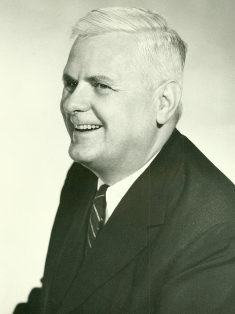
\includegraphics[height=2.0in]{images/alonzo_church.jpg}
  \end{center}
  \caption{阿隆佐·邱奇}
\end{wrapfigure}

由于“有效过程”的提法是一个非形式的、直观的概念,而“算法”的提法是一个精确的形式化的数学概念,很早就有人提出后者可以取代前者。
这正是\gls{邱奇论题}的实质内容\cite{KleeneSC1952}, 该论题断言,任何人们想称之为“有效”的过程,都已经可以通过一些适当编程的图灵机来完成。

现在,严格地说,到目前为止所描述的所有讨论都是完全形式化的;它们发生在命题和产生规则的逻辑和数学宇宙中。从某种意义上说,它们都是“软件”。
然而,有趣之处主要集中在这样一个事实上:像“机器”或“有效”这样的术语具有非数学的内涵,这些内涵都从属于自然物质现象的外部世界。
事实上,正如我们已经注意到的,图灵自己设计的数学机器是从现实世界的现象中抽象出来的,一个人在进行计算。
这种暗示如此不可抗拒地传达出, 如果人类精神活动的\emph{这一}方面可以“机械化”,为什么其他方面不可以呢? 为什么不可以是全部呢?
同样地,如果心理过程,包括在物质大脑中发生的事情(也即在硬件中)可以完全形式地表示,
为什么不能有其他类型的物质系统(也即其他硬件)可以做与大脑相同的事情?
虽然还在胚胎阶段,在这里,我们看到了,“人工智能”最广的推论,以及许多其他的意涵。

但是,一旦我们承认“机器”或“有效”这样的词具有物质意义,我们就离开了数学的世界,进入了(最广义的)物理世界。正如我们已经提到的,图灵机是“纯软件”,
而物理学则相反,是“纯硬件”。因此,无论是好是坏,我们引入了硬件和软件之间的根本区别,它本身并不是我们开始时所使用的形式理论的一部分;同样,它也不是物理学的一部分。
正如我们将要看到的,这种区别是至关重要的,但是也是隐蔽的,藏在包罗万象的总称“机器”中。从马丁·戴维斯的《可计算性和不可解性》\cite{DavisM1958}一书中,
我们可以看到这种区别是如何悄无声息地出现的:

\begin{displayquote}
    我们怎么能排除某一天(也许是某个外星访客)给我们一个(也许是极其复杂的)设备或“神谕”来“计算”一个不可计算函数的可能性呢?
\end{displayquote}

这显然是在一个完全形式化的数学进展背景下提出的最具修辞性的反问句。但是我们在这里清楚地看到术语“机器”的模糊性,
它建立在真实硬件和逻辑软件之间的默认区别之上。

\begin{figure}[ht]
\centering
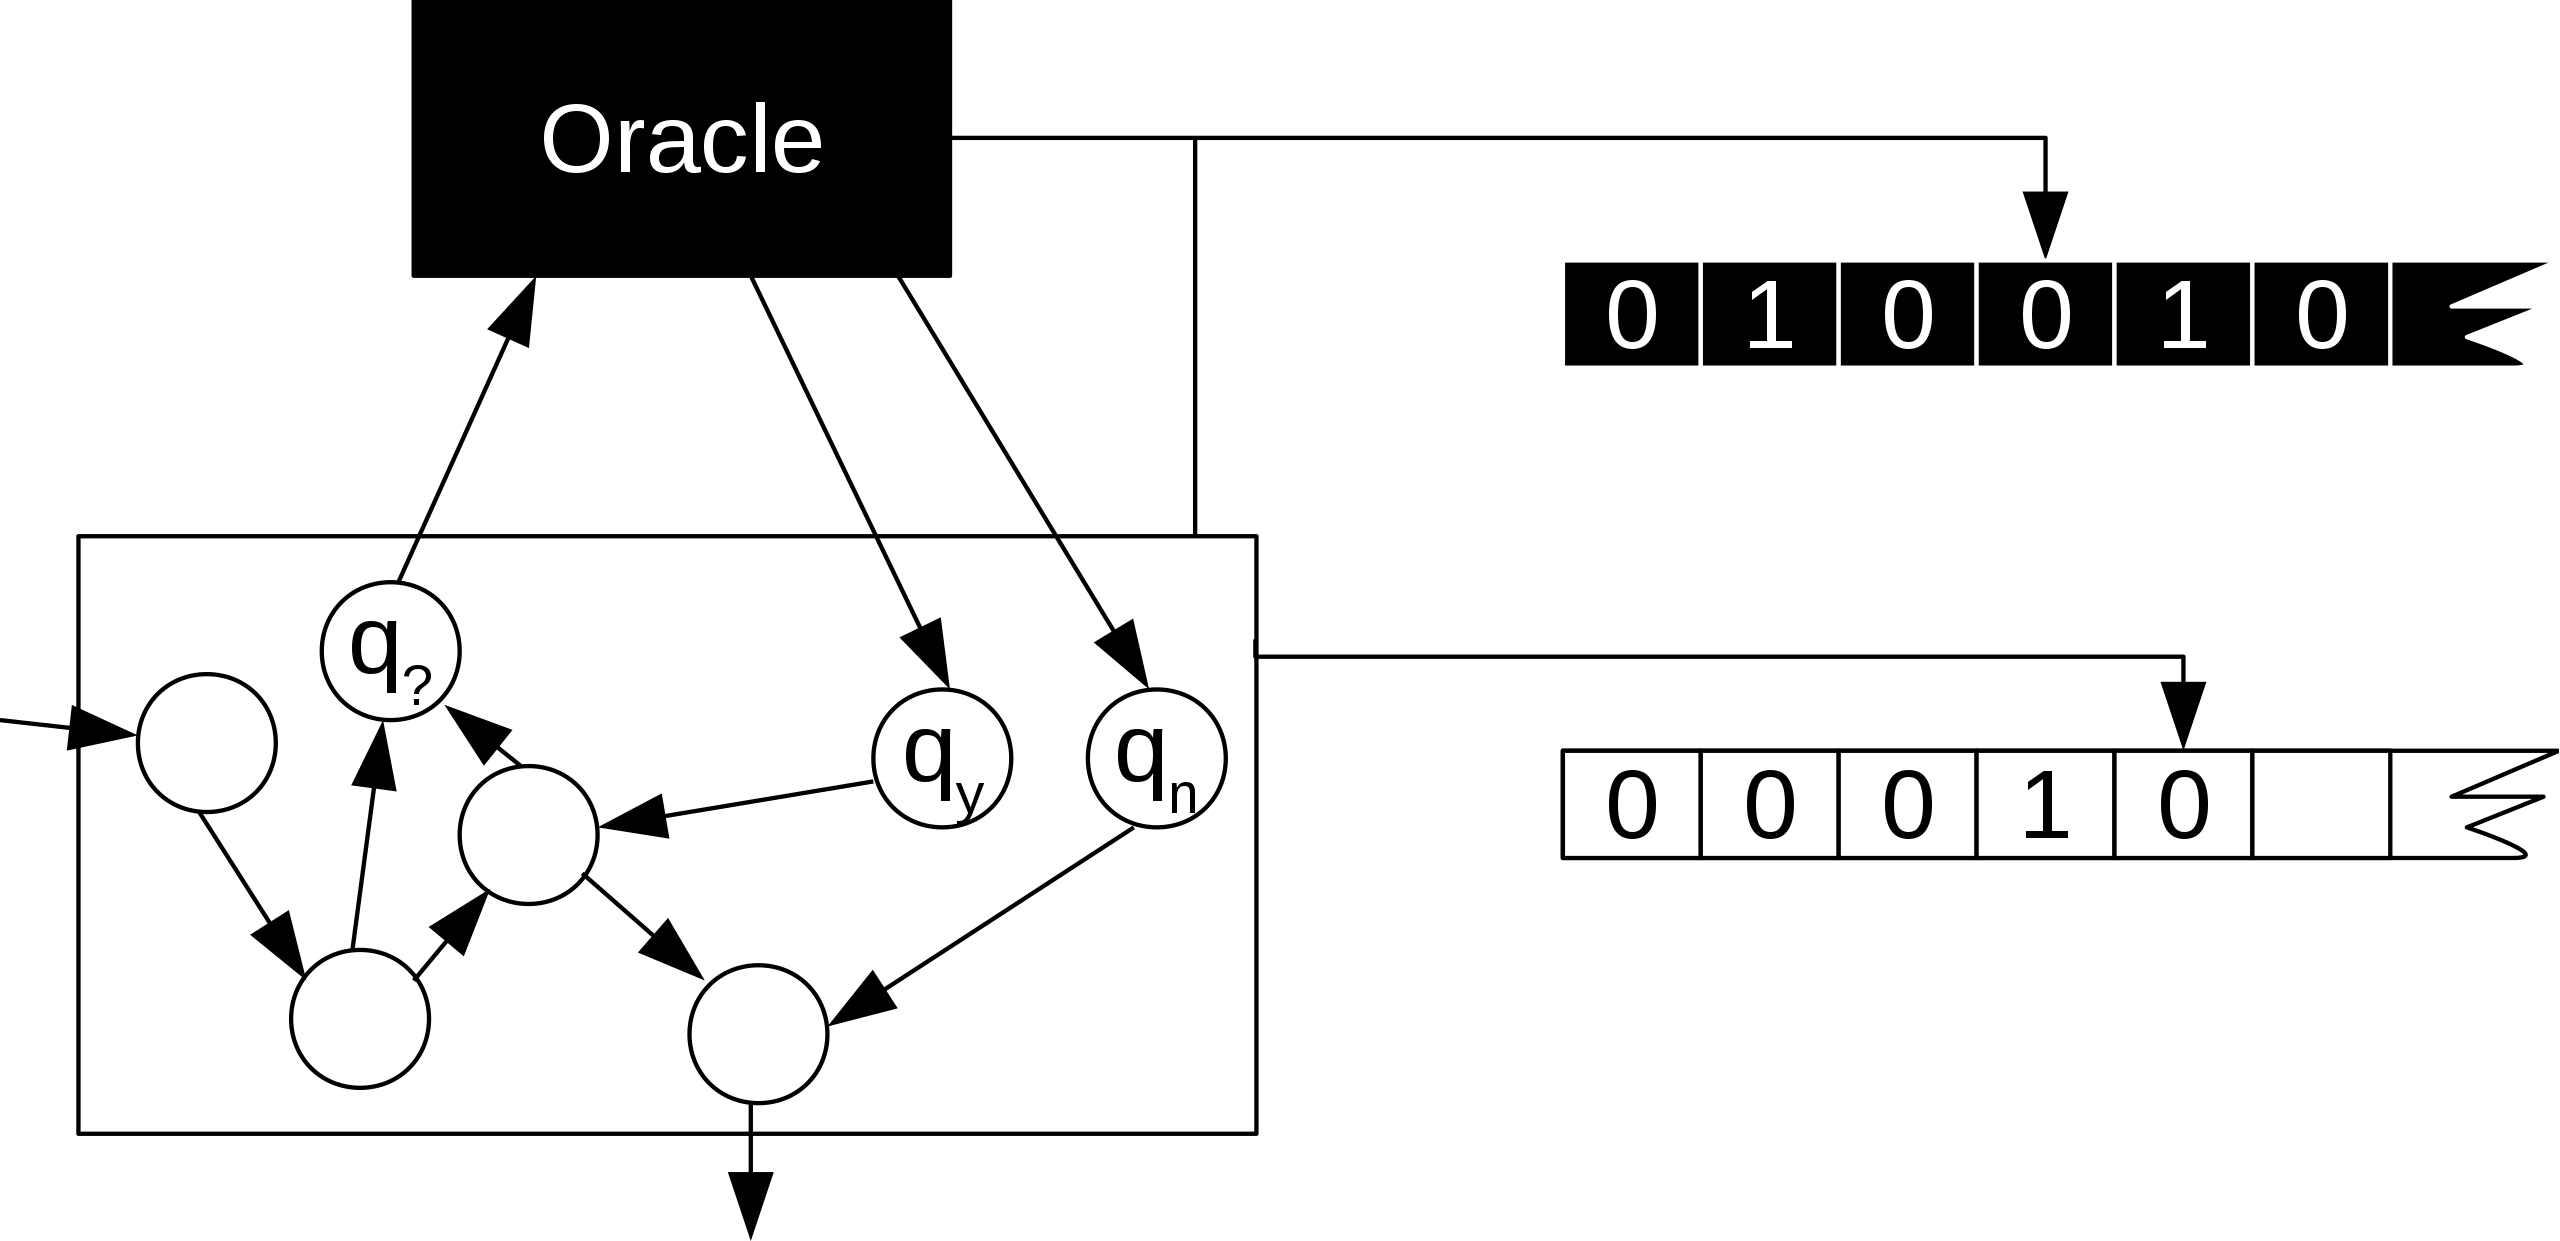
\includegraphics[height=2.0in]{images/turing_machine_oracle.png}
\caption{\gls{神谕图灵机}}
\end{figure}

长期以来,作者一直为这一问题的深层认识论的结论所困扰\cite{RosenR1962}。特别是,一旦我们承认“硬件”或物质系统进入我们的讨论(正如我们已经指出的那样,这从一开始就是明确无误的意图),
那么“有效过程”的概念会发生什么变化呢?很久以前\cite{RosenR1962},我考虑的问题是邱奇论题在这个新的背景下意味着什么。
特别地:邱奇论题是否是对物质本性的一个基本限制呢(类似于热力学定律排除了\emph{永动机}),或者相反? 如果邱奇论题可以被自然过程破坏,那么递归性又会怎么样呢?

在这里回顾一下先前论点的要点可能是有用的。假设我们有一个物理系统 $S$(也许是戴维斯的外星“计算机”)。它的行为受到物理定律的支配,我们通过实验来了解这些定律。
一个典型的实验要么对系统做一些事情(例如,从外部扰动它),要么让系统对其环境做一些事情,然后观察或测量结果。显然,实验者的干预和测量的结果都是物质事件。
事件是由数字来描述或刻画其特性的,其数值是由应用的合适的量表来决定的\cite{RosenR1978}。为了简单起见,假设我们的实验干预 $\alpha$ 拥有的属性是这样一个数值 $r(\alpha)$,
而我们系统的结果行为由另一个这样的数字刻画。通过这种方式,我们的实验者可以生成一个数值表,它定义了一个从数字到数字的函数 $f$。 \begin{equation} r(\alpha) \mapsto \beta\end{equation}

读者将会认识到,这个过程以典型输入输出的方式刻画了我们系统 $S$。函数 $f$ 的形式,清楚地告诉我们支配 $S$ 行为的规律。毕竟,这就是科学实验的全部功用。

这个实验过程在某种意义上是有效的。事实上,正如我们将在下面详细论述的那样,物质世界(例如,在系统 $S$ 中)的事件序列是由因果关系所支配的,这些因果关系将它们联系在一起,就像蕴涵关系将命题无可避免地联系在一起一样。
因此,如果我们的实验过程是可重复的(这意味着 $S$ 中相同的因果序列可以随意重建) ,那么邱奇论题必须意味着任何输入输出函数 $1$,正如我们已经描述过的任何物质系统 $S$,也必须是递归的或可计算的。
否则,系统 $S$ 将正是戴维斯向我们保证排除在可能性之外的那种“计算机”。

从这个角度来看,邱奇论题试图从软件(算法)的前提中得出关于硬件(物理学)的推论或结论。
冯·诺依曼关于“自我复制”的论点\cite{BurksA1966}体现了另一种众所周知的同样尝试。
在这里,我们的目的是从一个关于计算的形式理论中学习关于物质系统(特别是有机体)的行为的一些东西。
不出所料,这类尝试风险极大,但如果能成功实现,回报将是巨大的。

\begin{figure}[ht]
\centering
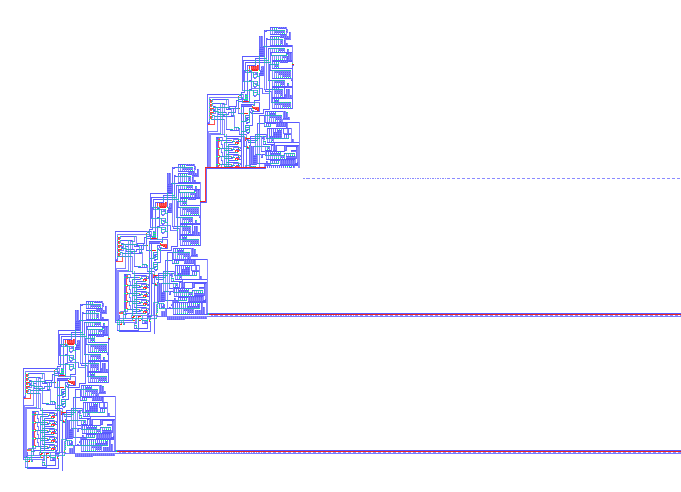
\includegraphics[height=2.0in]{images/self_reprod.png}
\caption{运行中的第一个为人所知的自复制机}
\end{figure}

至少,我们可能已经看到,在形式理论中引入“硬件”的概念将产生一些特殊的结论。而当我们试图把“软件”的概念引入物理学时,互补的结论就出现在另一方面。
然而,这些特殊的结论将告诉我们一些关于这两者的有趣事情。在本文的其余部分,我们将探索这种可能性。

\section{形式系统中的邱奇论题}

邱奇论题的实质是,把任何形式系统中的逻辑推理与字符串处理等同起来。反过来,字符串处理或字处理是一种纯粹的语法活动。
当然,字符串处理正是图灵机所做的。尽管如此,从表面上看,这似乎是一个非常强的、或许有些过于强的条件,
它要求形式系统中的每一个推理,都应该只用语法项来表达;也就是说,从前提到结论的每一个步骤,都应该完全通过,对这些编码了的命题的符号进行操作来实现。

然而,我们可以有一个相当有力的理由来支持这个看起来不太可能的论题。
它源自于一种形式化的趋势,这种趋势始于欧几里德,随着非欧几何的发现(作为形式系统,和上帝赋予的欧氏几何一样,是一致的几何学),
以及发现朴素集合论中悖论时的绝对绝望,这种混乱成为了一个紧迫问题。
大卫·希尔伯特开创的形式主义对这种情况的回应,恰恰是要清空数学的任何语义内容,辩称这些不必要的语义,是困难的根源。
实际上,这把所有的数学变成了一种游戏,在这种游戏中,无意义的符号按照(一种有限的)任意语法规则来处理。
事实上,希尔伯特形式主义的全部意义,在于创造一个除了语法以外什么都没有的系统。

\begin{figure}[ht]
\centering
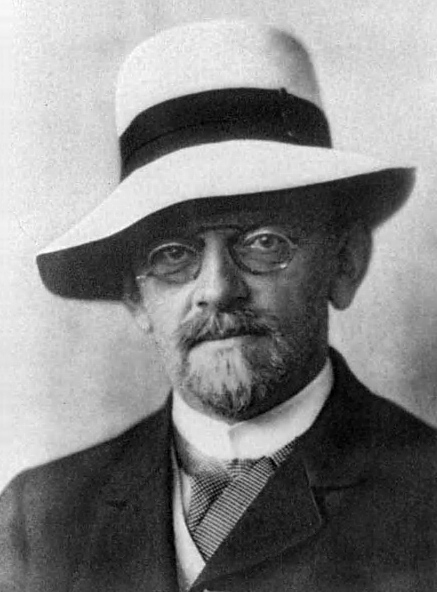
\includegraphics[height=2.0in]{images/hilbert.jpg}
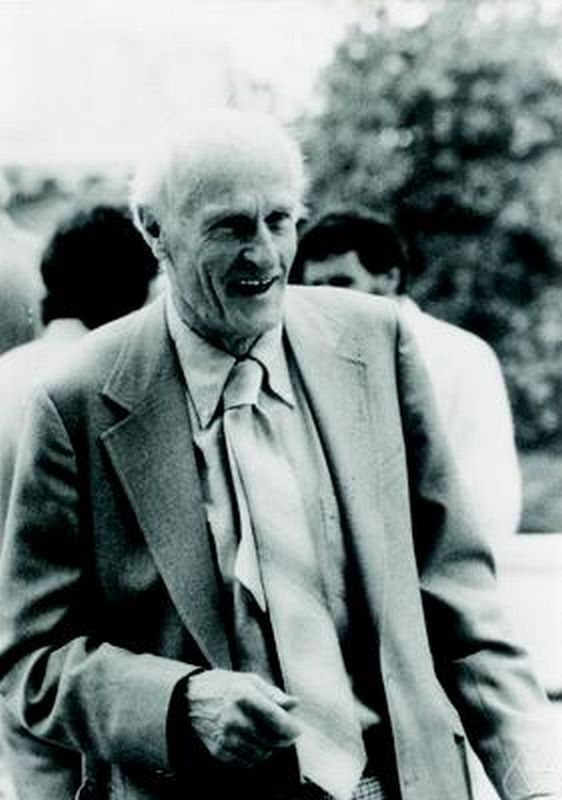
\includegraphics[height=2.0in]{images/kleene.jpg}
\caption{大卫·希尔伯特;斯蒂芬·科尔·克莱尼}
\end{figure}

或许,这种形式主义计划最清晰的陈述是由克莱尼给出的\cite{KleeneSC1952}

\begin{displayquote}
这一步(公理化)将不会完成,直到所有的未定义的性质或理论的技术性术语已表示成公理,它们对定理的推演是重要的。
然后应该有可能应用演绎法,把技术术语当作没有意义的单词。
因为,说它们对于定理的推导具有必要的意义,而不是说它们是从支配的公理中衍生出来的,
就等于是说,对于演绎来讲,它们并不都是可以用公理来表达重要性质的。
当技术性术语的含义因此被忽略了,我们就达到了形式公理学说的立场……
因为我们已经完全从内容中抽象出来,只留下形式,我们说原始理论已经形式化了。
在这种结构中,理论不再是一个有意义的命题系统,而是一个作为词序列的句子系统,这些词序列依次是字母序列。
我们只是参照形式来说,哪些单词组合成句子,哪些句子是公理,哪些句子是其他句子的直接后果。
\end{displayquote}

显然,这里的想法是,总是可以用语法替换语义(“意义”),从而在逻辑上没有信息丢失;
任何涉及语义的推理,在形式化中都有纯粹的语法映像。

在这样的一个形式系统中,我们首先认为公理是真的。这种真的概念是可传递的;
如果公理为真,那么通过将系统的推理规则应用于它们而获得的符号序列也是如此;因而,真从公理传递到定理。
到目前为止,我们从来不需要从外部引入“真”的概念到系统中,就像从前一样;我们只是在推演的过程中构造真的命题(定理)。

\begin{figure}[ht]
\centering
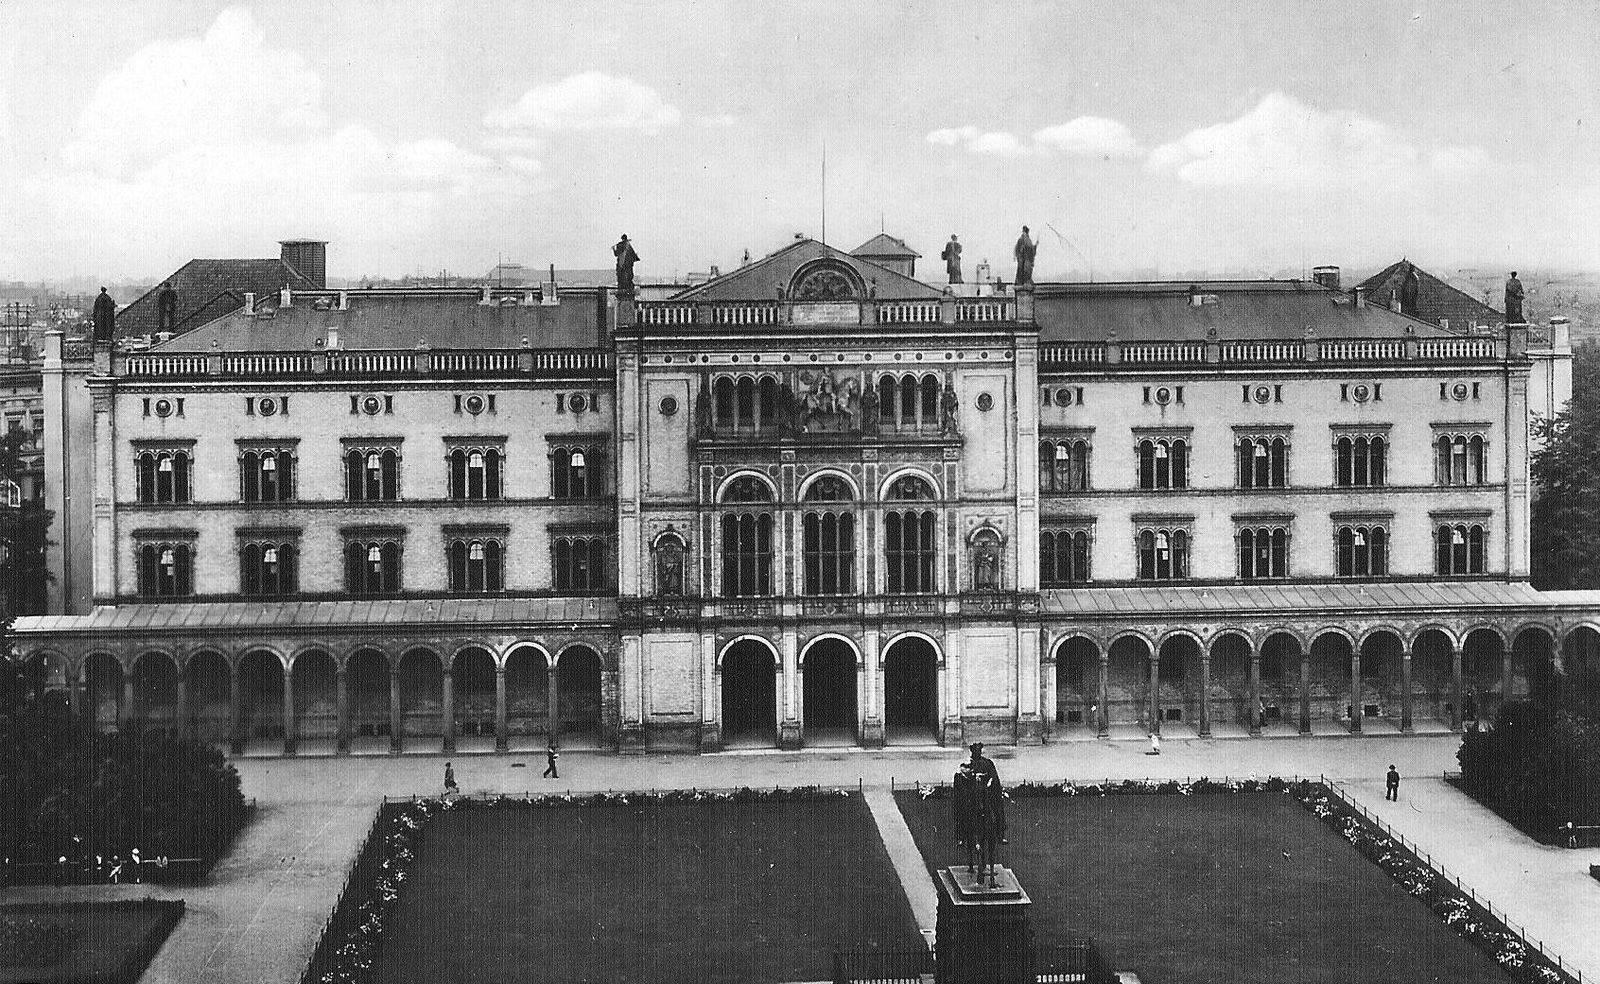
\includegraphics[height=2.5in]{images/konigsberger_university.jpg}
\caption{哥德尔不完备性定理最早于 1930 年 9 月在柯尼斯堡大学的一个学术会议上发表}
\end{figure}

哥德尔著名的定理\cite{GodelK1931}中所包含的麻烦,源自于试图将这种内部真理的构造性概念与形式算术中预先赋予的外部真值进行比较;正如哥德尔所示,它们并不匹配。
此外,看待图灵可判定性定理\cite{TuringA1937}的一种方式是,在给定的形式化中,没有内部推理机制来决定一个命题是否是一个定理(即,是真的)。
因此,我们知道,形式主义计划,其中只有纯粹的语法推论是允许的,是过于贫乏的,甚至不足以支撑数论。
也就是说,我们要么允许一些“非形式”的推理过程进入我们的系统,根据哥德尔定理,这些程序甚至在原则上都不能简化为语法; 要么永远把我们自己限制在数论的片段中。
这种“非形式”的推理过程是邱奇论题所不允许的,它们是无效的。

让我们用更熟悉的术语来讨论上述问题。 在普通(“柏拉图式”)数学中,它同时具有语法和语义学的方面,
我们知道,如果我们给定一个集合 $S$ ,通过规范结构可以从 $S$ 构造出许多其他集合。
例如,我们有幂集 $2^S$ ,我们有 $S$ 生成的自由代数结构(半群,群等) ,我们有从 $S$ 到 $S$ 的所有映射的集合 $H(S, S)$ ,
我们有笛卡儿积 $S \times S$ ,等等。
这些相关的集合赋予我们推理能力,这些能力具有逻辑关系的力量,但这些支配 $S$ 的数学系统的形式推演律,并不必然有足够的表达力。
例如,如果 $Q: S \mapsto S$ 是一个自同构(即 $H(S, S)$ 的一个元素) ,对 $s \in S $,我们可以说 $Q(s) = s^{\prime}$ 在 $s$ 和 $s^{\prime}$ 之间建立了一个蕴涵关系。
但是,这种“蕴涵”不一定与我们可以从支配系统的产生式规则中得出的结论相一致,也就是说,不必仅仅遵循系统的语法。
如果两者是一致的,可以说我们的 $Q$ 在系统中是可计算的;否则,就是不可计算的。在后一种情况下,根据邱奇论题,我们不得不说映射 $Q$ 是无效的。
但是很明显,如果 $Q$ 有意义或存在,一旦它被赋予给我们,它就是有效的。

在形式系统的“全软件”的世界中,我们当然可以用任何喜欢的方式来限定自己。
因此,我们可以不允许我们自己拥有任意的自同构 $Q$,它是不能表示成纯粹的语法项的。
在这样一个世界里,也只有在这样一个世界里,邱奇论题才能不受限制地成立。
当然,这样一个正式的世界是否有趣,是另一个问题。正如我们将看到的,当我们允许“硬件”进入我们的世界时,情况会变得更加糟糕。

在讨论物质系统之前,我们应该先把形式系统中的命题编码到图灵机码带上,然后再把码带上的内容解码成系统中的命题。
很明显,在编码和解码方面,我们可以按照通常的直观意义使用“有效”一词;例如,我们熟悉的哥德尔编码,
显然是从语法到算术、然后再回来的有效映射。事实上,通过证明一个过程在某些形式系统中是有效的,或者说是递归的,
我们可以清楚地将编码、计算和解码结合到一个单独的图灵机中,这个机器可以完成所有三个步骤。
然而,我们在这里只是记下,编码和解码在逻辑上彼此不同,也不同于实际计算;
如果它们在某种意义上是“无效”的,那么邱奇论题可能会失败,即使计算本身是完全递归的。

\section{蕴涵与因果}

正如我们已经看到的,在形式系统的领域,邱奇论题辨析了“有效过程”的直觉概念与纯粹的语法观点下的字符串处理。

\begin{figure}[ht]
\centering
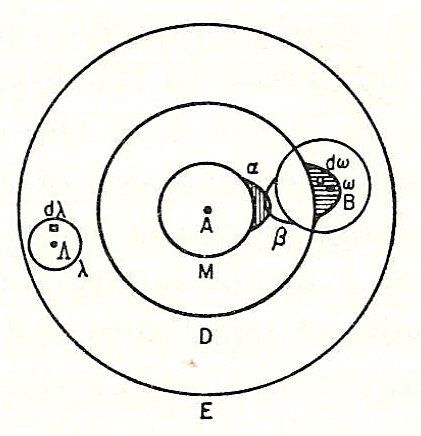
\includegraphics[height=2.5in]{images/boltzmanns_molecule.jpg}
\caption{玻尔兹曼设想的由原子构成的分子}
\end{figure}

也就是说,任何可以在系统内“有效地”执行的蕴涵,都可以通过一套有限的产生规则来执行,这套规则操作于从一个有限字母表中取出的有限的符号串。
我们还指出,当我们在处理物质世界时(相对于形式的数学和逻辑),蕴涵的观念被因果关系的观念所取代。
尽管如此,我们仍然可以保留“有效”过程的想法。 在这种情况下,邱奇论题意味着任何因果序列都可以用相应的递归过程来表示;
也就是说,任何因果序列都可以用纯粹的语法手段来描述。 如果这是真的,它当然会严重限制物理学的发展。
是否自然法则本身可以表达成纯粹的语法项,或者它们是否可以拥有一个内在的语义组成部分不能被有限形式化,问题绝不仅仅限于此。
值得注意的是,数学中的形式化(即纯粹的语法)与理论科学中的类似趋势是完全平行的。
事实上,原子论(或者现在的“基本粒子”理论)的全部推动力是将所有物质过程简化到终极组成单元的运动,而没有任何内部结构(“意义”),
只拥有瞬时位置(“构型”)和位置的瞬时导数。推动这些终极单元的力量与形式系统中的产生式规则完全相同。
因此,一个物质系统在给定力的影响下所追踪到的路径或轨迹是形式定理的类比,以初始条件为公理。
物质系统中事件之间的因果关系可以与描述这些事件的命题之间的蕴涵关系相联系的观点是理论科学的必要条件。
事实上,过去被称为自然法则的信念要求:
\begin{enumerate}[label=(\alph*)]
\item 我们在外部世界中感知到的事件序列不是任意的或异想天开的,而是受到明确规则的支配(这就是因果关系);
\item 这些规则可以清楚地表达出来,以便人类头脑能够理解。
\end{enumerate}
综上所述,自然法则的这种表述精确地断言,物质系统中的因果关系可以被引导到一个形式化的(终极的,数学的)命题系统的一致性蕴涵关系中。

这种情况可以最简洁地用图式一来表示(参见图9)。

\begin{figure}[ht]
\centering
\begin{tikzpicture}
[round/.style={rounded corners=1.5mm, minimum width=1cm, inner sep=2mm, above right, draw, align=center, text width=7mm}]
    \node[round] (N) at (0,0) {自然系统};
    \node[round] (F) at (6,0) {形式系统};
    \path[draw, thick, bend left=-45]
        ($(N.east)+(0,-1.0)$) edge[->] node[near start] {\hspace{+6em}\ding{193}编码} ($(F.west)+(0,-1.0)$);
    \path[draw, thick, bend left=-45]
        ($(F.west)+(0,1.0)$) edge[->] node[near start] {\hspace{-6em}\ding{195}解码} ($(N.east)+(0,1.0)$);
    \path[draw, thick, bend left=-45]
        ($(N.west)+(0,+0.8)$) edge[->] node {\hspace{-3em}\ding{192}因果} ($(N.west)+(0,-0.8)$);
    \path[draw, thick, bend left=-45]
        ($(F.east)+(0,-0.8)$) edge[->] node {\hspace{+3em}\ding{194}蕴涵} ($(F.east)+(0,+0.8)$);
\end{tikzpicture}
\caption{图式一}
\end{figure}

我们说,当以下的交换性成立时,图表左侧的自然系统和右侧的形式系统之间存在一种建模关系:\begin{equation} \Circled{1} = \Circled{2} + \Circled{3} + \Circled{4}\end{equation}

也就是说,无论我们是仅仅作为观察者坐在那里,观察自然系统中事件的展开序列,还是我们
\begin{enumerate}[label=(\alph*)]
\item 将自然系统的某些性质编码到形式体系;
\item 然后利用形式系统的蕴涵结构导出定理;
\item 再将这些定理解码成关于自然系统本身的命题(预测)
\end{enumerate}
我们都得到了同样的答案。当图表交换时,我们在自然系统的因果特征和形式系统的蕴涵结构之间建立了一个一致性。
我们可以说形式系统是自然系统的模型,或者说,自然系统是形式系统的实现。

这些小图表本身包含许多丰富而重要的认识论属性,我们不能在这里进入;要进行更全面的讨论,请参阅\cite{RosenR1985}。

一旦我们建立了一个形式的系统,作为某种自然过程的模型,我们就离开了科学的领域,进入了数学的领域。
然后,我们可以像对待其他任何形式系统一样对待模型。特别是,我们可以看看它纯粹的语法方面,
我们可以立即辨认出邱奇论题里的“有效”过程,并问这些过程是否耗尽了系统本身的蕴涵性资源。

通过这种方式,我们可以构建一个纯语法的原本的自然系统的“机器”模型,如 图10 所示。

\begin{figure}[ht]
\centering
\begin{tikzpicture}
[round/.style={rounded corners=1.5mm, minimum width=1cm, inner sep=2mm, above right, draw, align=center, text width=7mm}]
    \node[round] (N) at (0,0) {自然系统};
    \node[round] (F) at (4,0) {形式系统};
    \node[round] (M) at (8,0) {机  器};
    \path[draw, thick, bend left=-45]
        ($(N.east)+(0,-1.0)$) edge[->] node[near start] {} ($(F.west)+(0,-1.0)$);
    \path[draw, thick, bend left=-45]
        ($(F.west)+(0,1.0)$) edge[->] node[near start] {} ($(N.east)+(0,1.0)$);
    \path[draw, thick, bend left=-45]
        ($(F.east)+(0,-1.0)$) edge[->] node[near start] {} ($(M.west)+(0,-1.0)$);
    \path[draw, thick, bend left=-45]
        ($(M.west)+(0,1.0)$) edge[->] node[near start] {} ($(F.east)+(0,1.0)$);
    \path[draw, thick, dotted, color=lightgray, bend left=-45]
        ($(N.south)$) edge[->] node[near start] {} ($(M.south)$);
    \path[draw, thick, dotted, color=lightgray, bend left=-45]
        ($(M.north)$) edge[->] node[near start] {} ($(N.north)$);
    \path[draw, thick, bend left=-45]
        ($(N.west)+(0,+0.8)$) edge[->] node {\hspace{-3em}因果} ($(N.west)+(0,-0.8)$);
    \path[draw, thick, bend left=-45]
        ($(F.east)+(0,-0.8)$) edge[->] node {\hspace{+3em}蕴涵} ($(F.east)+(0,+0.8)$);
    \path[draw, thick, bend left=-45]
        ($(M.east)+(0,-0.8)$) edge[->] node {\hspace{+5em}字串处理} ($(M.east)+(0,+0.8)$);
\end{tikzpicture}
\caption{图式二}
\end{figure}


我们只看外侧的两个系统,忘记原本的模型,这个模型现在在两者间扮演一种“转换器”的角色。

但是,当我们这样做时,必须明确注意以下几点:
\begin{enumerate}[label=(\alph*)]
\item 它们之间的编码和解码箭头(图式二中的虚线箭头)在任何形式意义上都不能被描述为有效的;
\item 这些编码和解码箭头只涉及居最右的边框中的机器的输入和输出字符串;
\end{enumerate}
这两个观察结果都很重要。我们将依次简要地讨论它们。

\begin{figure}[ht]
\centering
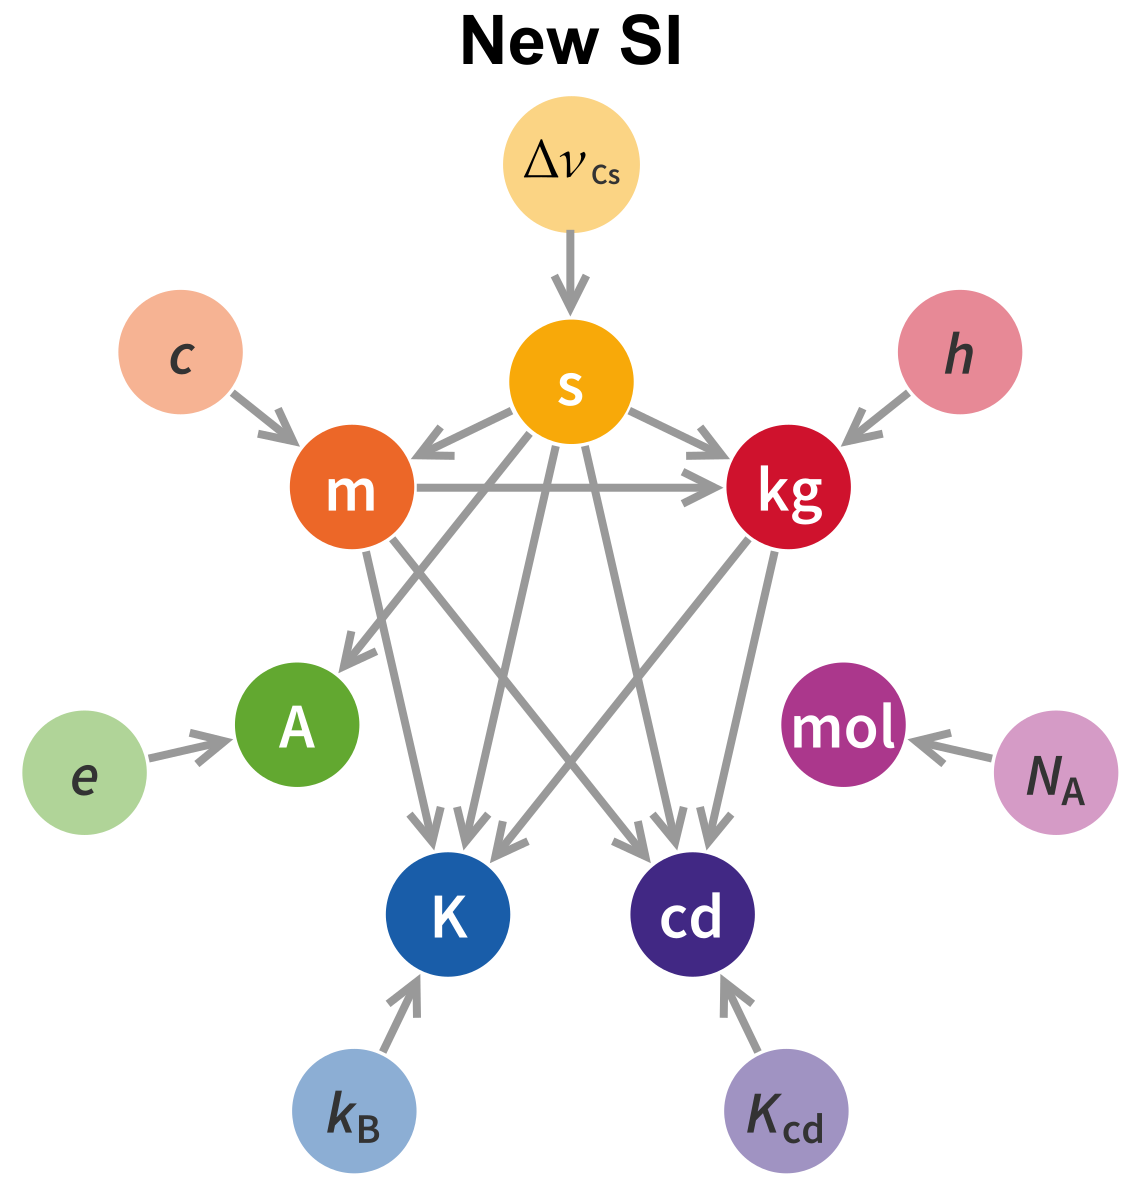
\includegraphics[height=2.5in]{images/unit_relations_SI.png}
\caption{测量问题:SI 2019 中基本量和物理常数之间的关系}
\end{figure}

在将邱奇论题应用于形式系统时,我们注意到上述相应的编码和解码箭头本身代表形式过程,实际上可以合并到论题本身。
然而,当我们想要比较一个受因果关系支配的自然系统和一个受蕴涵支配的形式系统时,情况就不一样了。
编码工具,或转换器,现在本身就是物质系统;也就是说,是由因果关系而不是蕴涵所支配。
如上所述,它们(在最广泛的意义上)是仪表。因为这些仪表受因果关系支配,它们所做的任何事情在物质意义上都是有效的。
但是很明显,编码过程的形式化需要更多的模型;这反过来又需要它们自己的编码和解码过程,这就需要更多的模型,等等,一个无穷回归。
正是这一事实使物理学中的“测量问题”变得如此困难。
这个潜在的无穷回归是否可以在某个有限点终止的问题是一个关于世界本质的深刻的认识论问题,与还原论这样的事物有着密切的联系。
我们当然不能在这里进入这样的问题;我们只是假设从自然世界到输入码带的一套仪表或其他转换器是给定的,
并且可以相对于这些编码对邱奇论题进行调查(然后,通过假设,在物质意义是有效的)。

我们的第二个观察在认识论上也很重要。它说,一个物质系统的所有相关特征,以及它最初被编码进去的模型的所有相关特征(参见图式一) ,
都被表示为输入字符串,由一台其结构本身不编码任何东西的机器处理。也就是说,控制这些机器操作的规则,以及字符串处理系统本身的整个推理结构,
与被编码的物质系统毫无关系。唯一的要求是,在输入字符串的编码和结果输出字符串的解码之间保持必要的交换性,如上文第1节所述。
正如我们将看到的,这就是模拟的本质。

我们已经注意到,邱奇论题相当于断言,所有的因果关系,可以表达成纯粹的语法项。
我们现在可以更明确地阐述这个命题: 相对于将自然系统的任何特定编码转化为输入字符串,字符串处理机器本身不能对物质系统的任何方面进行编码。
也就是说,机器的“硬件”必须完全独立于生成要处理的字符串的“硬件”。 如果不能做到这一点,那么邱奇论题就不可能是正确的。

鉴于上述,邱奇论题断言,对所有物质过程,图灵机构成了一类通用的模拟器。 这里有两个问题要问: (a)这是真的吗? (b)如果是,那意味着什么?

\section{邱奇论题在物理上是正确的吗?}

前面几节论证的结果如下。大自然为我们提供了大量的物质过程,我们称之为“有效”。
这些过程(我们假设)受因果关系支配,而不像在形式系统中那样受蕴涵或生成规则支配。
在这样的术语中,邱奇论题可以表达如下:给定任何如此的过程,关于自然系统的适当命题,我们可以编码生成它到一个图灵机的一组输入码带上;
而相应的输出码带可以被解码,从而完美地模拟了有关的过程。同样地,邱奇论题断言,所有关于物质过程的“信息” ,因此所有的自然法则,
都可以用纯粹的语法项来表达。

我们从哥德尔定理中知道,足够丰富的形式系统总是包含一些不能从语法上得到的推论。
更具体地说,给定任何命题编码方案,它将系统的命题编码到图灵机的输入码带上,都将有系统的“真”的命题,它不会出现在任何输出码带上。
因此,建立这种推论为“真”的过程是无效的;它们原则上,不能被任何图灵机,在给定的编码上模拟。
当然,我们可以随时改变编码,但这不会改变哥德尔的结论。

因此,在形式系统中,我们已经发现纯粹的语法编码在某种意义上会丢失信息。
因此,丢失的信息必须属于原始推理结构中一个不可规约的、不可形式化的语义成分。
通过改变编码,我们可以在一定程度上改变这个语义信息所在的位置,但是我们不能消除它。

就其本身而言,哥德尔的这个结果与邱奇论题的物理真实性无关,因为它是一个纯粹形式上的结果。
但它实际上暗示了邱奇论题的物理源泉如何可能被证实或证伪。

正如我们在上面看到的,我们比较物质过程和形式过程的方式是通过建立建模关系,如上面图式一所示。
物质系统的形式化模型是非常好的形式化系统,其推理结构从定义上反映了被建模的自然系统中的因果过程。
因此,如果一个模型,以这种方式产生,应该属于哥德尔论证的范围,这将至少是强有力的证据,证明邱奇论题,作为一个物理命题,是虚假的。
换句话说,可能存在能够有效计算的非递归函数的物理过程。这也意味着自然法则不能完全用语法项来表达。

因此,显而易见要寻找的是一个物质系统的模型,它作为一种形式体系足以“做算术”。
不幸的是,物理学提供的作为纯粹物理系统模型的形式体系极其贫乏,可以简单地认为是形式系统。
但是,正如我们在其他地方所争论的,这些形式体系事实上是高度非通用的,不足以描绘像有机体这样的物质系统\cite{RosenRinpress}。
表达这种非通用性的一种方式,就是精确地表达它们对因果结构的映像。当这种非通用性被移除的时候,一类新的(潜在)模型就被提出了,其中因果结构的映像更加丰富和复杂。
因为,正是因果结构的形式化映像是邱奇论题的核心,我们可能会在这些形式体系中发现许多因果有效的过程,但在数学上是无效的。
这就意味着这些系统的行为必须包含一个不可约的语义成分,一个与系统的复杂性密切相关的成分。

约翰·米希尔很久以前就采取了不同的方法\cite{MyhillJ1966}。
他能够证明,模掉一些理想化的测量和性能公差,已经有经典的模拟设备(模拟计算机),可以“计算”非递归函数。
这样的系统将因此已经表现出任何纯粹的语法编码无法预测的行为,因此也将有一个不可规约的语义内容。

最后,我们已经提到,牛顿粒子力学,以及最近基于基本粒子的统一物理理论,本身就是一种试图用纯语法项来表达自然法则的尝试。
由于任何物质系统都是由这些“无意义”(即无结构)的基本单元组成的,这些理论本质上断言,要理解任何这样的系统的任何行为,
就足以用这些子单元及其相互作用来描述它。如前所述,这就是还原论的本质。

在这些术语中,熟悉的拉普拉斯精灵是一个纯粹的语法概念: 如果他可以存在的话,就是邱奇论题的体现。
事实上,由于我们已经指出的原因,他不可能存在(或者至少不可能作为一个由粒子构成的物质系统存在)。
但是即使他能够存在,他也是一个非常糟糕的生物学家,例如,有机体和一般的开放系统,都在不断地转动它们的组成粒子。
因此,即使要找到一个有机体,更不用说及时跟踪它,他也需要用系统内不可形式化的其他(语义)信息来补充纯粹的语法信息。

因此,由于种种原因,我们有理由相信邱奇的命题作为一个物理命题是失败的。
然而,正如我们已经看到的,从物质方面去陈述和分析邱奇论题,涉及到理论科学的一些最深刻和最基本的方面。

\section{模拟的角色}

我们已经在上面提到了图灵机的使用,它既是对物质世界的隐喻,也是对那个世界的有效描述。
在这两种情况下,虽然以不同的方式,我们试图从纯粹的语法形式中得出关于物质过程的结论。
在最后一节中,我将非常简要地考虑一个著名的例子: 冯·诺依曼的“自复制自动机”\cite{BurksA1966}\cite{ArbibMA1988}。

冯·诺依曼论证的基础是根据图灵关于通用模拟器(计算机)的论证推断“通用构造器”的存在。
在纯形式方面,冯·诺依曼构建了一个由互通图灵机组成的宇宙(“元胞空间”),这些机器排列成规则的几何阵列,就像多细胞生物中的细胞,或者大脑中的神经元,或者晶体中的原子。
每台机器都与数组中最近的邻居通信。按照显而易见的方式,阵列作为一个整体在时间上改变“状态”。
问题是一些子阵列(“铺嵌自动机”)能否在其补(its complement)上诱导出某些有趣的行为,这些行为可以解释为构造、复制、增长、发展、进化等等。

同时,冯·诺依曼清楚地相信“通用构造函数”可以作为硬件存在。
他设想给图灵机配备传感器,这样它就可以“读取”蓝图,并配备效应器,这样它就可以从周围环境中提取物理组件,并按照被读取的蓝图的指示组装它们。
(在这个上下文中,“效应器”是从数字到实物的转换器,例如,“反射计” — an “inverse meter”)
这里的想法是—计算和构造都是算法过程,因此任何对一个真实(true)的东西都必须对另一个真实。

冯·诺依曼还认为元胞空间不仅仅是形式上的构造,实际上还包含了真实世界的构造器和它行为的模型。在这一点上,他默认了邱奇论题的最强形态。

我们已经在其他地方\cite{RosenR1985}论证,根据因果关系,从一个形式的通用计算机的存在导出一个物质的普遍构造器的任何推论都是没有根据的。
在这个论证中,我们基本上表明,没有内在的方法可以区分那些编码了“真实世界信息”的输入字符串和那些没能编码的输入字符串。
因此,没有办法区分可以声称模拟“真实世界”进程的计算和没有实现这种模拟的计算。

反过来,我们也可以看到,邱奇论题的虚假性意味着物质过程的某些方面不能被任何给定的编码来形式化。
因此,存在 (a)没有物质对应物的形式结构,反之,(b)没有形式对应物的物质构造。因此,在这两个方面,冯·诺依曼的论点都没有实质内容,
仅仅涉及到“自动机”(或“机器”)和“构造”这两个术语常见的模棱两可。

这些考虑表明,不受限制地从形式系统外推到物质系统是多么危险。
危险恰恰产生于这样一个事实,即计算只涉及模拟,这使得在物质系统中的因果过程和模拟器中的推理过程之间不能建立一致性。
因此,我们恰恰缺乏这种外推所需的编码和解码的基本特征。因此,尽管形式化模拟具有重要的实用价值和启发性价值,
但它们的理论意义却受到严格限制,使用时必须格外谨慎。

当然,在这个简短的篇幅里,我们无法触及邱奇论题的许多其他分支。正如我们已经看到的,它的主要作用是将形式系统中的语法部分和非语法部分区分开来;
当形式系统也是物质系统的模型时,邱奇论题对因果关系也做了同样的事情。事实上,这篇论文提出了一系列关于自然法则、因果关系、建模以及形式系统的物质实现的深刻问题。
它的中心特征是图灵机,将语法或字符串处理的本质体现在一个单一的、概念丰富的包中。即使(我相信)邱奇论题失败了,它也是以一种最富教育意义的方式失败的。
它对物质科学,尤其是生物学的影响,还没有开始探索。

\newpage
\phantomsection
\addcontentsline{toc}{section}{参考文献}
\bibliographystyle{ieeetr}
\bibliography{biblio/article}

\newpage
\phantomsection
\addcontentsline{toc}{section}{术语列表}
\printindex
\printglossaries

\end{document}




